\documentclass[a4paper,11pt,dvipdfmx]{ujarticle}
% パッケージ
\usepackage{graphicx}
\usepackage{url}
\input{layout}
% レイアウト指定を記述したファイルの読み込み

% タイトルと氏名を変更せよ．
\title{日本におけるデジタル化の状況}
\author{G685082026 山下遥大}

\begin{document}

\maketitle %ここにタイトルが入る

\section{ブロードバンドの整備状況}% ここから本文
% 節見出し: \section{}
% 本文(1)
%  参考文献の参照: \cite{}
%  図番号の参照： \ref{}
% を使う
% 文献データベースのキーワードは oecd と imd
% になっている．
OECDによるプロードバンド回線の普及に関する調査\cite{oecd}によると、
図\ref{fig:加入者数}に示すように、
日本における 100人あたりのモバイルプロードバンドの加入者数は190.5で、
第1位になっている。2位はエストニア
で、3位米国と続く。

\begin{figure}[htbp]
    \centering
    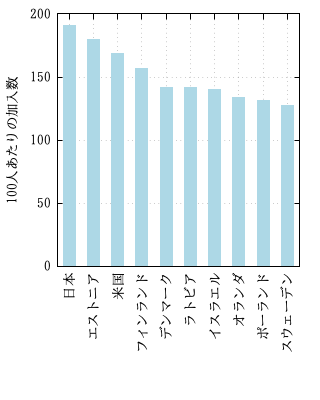
\includegraphics{fig21.png}
    \caption{光ファイバー回線の加入者数（100人あたり）}\label{fig:加入者数}
\end{figure}

\section{デジタル競争力ランキング}

国際経営開発研究所（IMID）の調査\cite{imd}によると、
表\ref{tbl:競争力}に示すように、日本のデジタル競争力のランキ
ングは調査対象の64カ国中、総合で28位。知識分野で25位となっている。

\begin{table}[htbp]
    \centering
    \caption{デジタル競争力ランキング（64カ国中）}
    \label{tbl:競争力}

    \begin{tabular}{|c|c|c|}\hline
        国 & 総合 & 知識  \\
        \hline
        米国 & 1位 & 3位 \\
        \hline
        香港 & 2位 & 5位 \\
        \hline
        スウェーデン & 3位 & 2位 \\
        \hline
        デンマーク & 4位 & 8位 \\
        \hline
        シンガポール & 5位 & 4位 \\
        \hline
        韓国 & 12位 & 15位\\
        \hline 
        中国 & 15位 & 6位 \\
        \hline
        日本 & 28位 & 25位 \\
        \hline
    \end{tabular}
\end{table}

\section{考察}

以上の調査結果から私が考えたこと
\begin{itemize}
    \item 日本は100人あたりのモバイルプロードバンドの加入者数が第1位になっているのに対し、デジタル競争力ランキングでは総合で28位となっていることから日本はモバイルプロードバンド回線以外の分野にも力を入れて取り組んでいくべきだと考えた。
    \item デジタル競争力ランキングの知識分野で、日本が他のアジア各国に遅れをとっていることからデジタルについて学びやすい環境作りを進めていくべきだと考えた。
    \item デジタル競争力を高めるにはなるべく多くの企業にITツールの導入することやAIや最新ツールを使いこなせる人材育成が必要だと考えた。
\end{itemize}

\bibliographystyle{junsrt}
\bibliography{exercise.bib}

\end{document}



% 図の挿入
% \includegraphics{}
% を
% \begin{figure}[htbp]
% \end{figure}
% で囲み
% \caption{}
% で図のタイトルを入れる．
% \label{}
% を使って図番号が参照できるようにする
% また，
% \centering
% で図が中央に来るようにする
% ーーー
% 節見出し(2)

% 本文(2)

% 表の挿入
% \begin{tabular}
% \end{tabular}    
% による表の記述を 
% \begin{table}[htbp]
% \end{table}
% で囲み
% \caption{}
% で表のタイトルを入れる．
% \label{}
% を使って表番号が参照できるようにする
% また，
% \centering
% で表が中央に来るようにする

% ーーー
% 見出し(3)
% 考察
%
% \begin{itemize}
% \end{itemize}
% を使って箇条書きで記述する

% ここに参考文献が入る
%